\documentclass{article}
\usepackage[utf8]{inputenc}
\usepackage{graphicx}
\usepackage{booktabs}
\usepackage{amsmath}
\usepackage{amssymb}
\usepackage[hidelinks]{hyperref}
\usepackage{geometry}
\usepackage{float}
\usepackage{xcolor}
\usepackage{listings}
\usepackage{enumitem}
\usepackage{natbib}
\usepackage{tikz}
\usepackage{pgfplots}
\usepackage{indentfirst}
\pgfplotsset{compat=1.17}

% Define colors for code highlighting
\definecolor{codegreen}{rgb}{0,0.6,0}
\definecolor{codegray}{rgb}{0.5,0.5,0.5}
\definecolor{codepurple}{rgb}{0.58,0,0.82}
\definecolor{backcolour}{rgb}{0.95,0.95,0.92}

% Set up code listing style
\lstdefinestyle{mystyle}{
    backgroundcolor=\color{backcolour},
    commentstyle=\color{codegreen},
    keywordstyle=\color{magenta},
    numberstyle=\tiny\color{codegray},
    stringstyle=\color{codepurple},
    basicstyle=\ttfamily\footnotesize,
    breakatwhitespace=false,
    breaklines=true,
    captionpos=b,
    keepspaces=true,
    numbers=left,
    numbersep=5pt,
    showspaces=false,
    showstringspaces=false,
    showtabs=false,
    tabsize=2
}
\lstset{style=mystyle}

\geometry{margin=1in}

\title{Railway Station Profit Analysis: \\ Statistical Assessment and Economic Interpretation}
\author{Statistical Analysis Project}
\date{\today}

\begin{document}

    \maketitle

    \begin{Resume}
        This report presents a comprehensive statistical analysis of annual profits for railway stations. The analysis includes key descriptive statistics (mean, standard deviation, median, and mode), identifies outliers in the profit data, and determines the most and least profitable years for each station. Beyond statistical calculations, this document provides detailed theoretical foundations for the applied methods and interprets the results within the broader context of transportation economics and infrastructure management. The methodology implemented in Python offers an interactive approach where users can specify which station they want to analyze, making this a valuable decision-support tool for railway network optimization.
    \end{Resume}

    \tableofcontents

    \section{Introduction}
    \indent Railway station profitability serves as a critical metric for transportation network management. Understanding the financial performance patterns of individual stations can inform strategic decisions about resource allocation, infrastructure development, and operational improvements. This project implements a statistical analysis tool that allows users to examine the profit patterns of any station in the network.

    The financial sustainability of railway stations represents a crucial element in the broader transportation infrastructure ecosystem. With increasing pressure on public transportation systems to become more economically self-sufficient while maintaining service quality, analyzing station-level profit dynamics provides essential insights for targeted interventions and policy development.

    \section{Objectives and Theoretical Foundations}
    \subsection{Project Objectives}
    The primary objectives of this analysis are:

    \begin{enumerate}[label=\arabic*.]
        \item To develop a robust statistical framework for analyzing railway station profitability
        \item To identify significant patterns and anomalies in annual profit data
        \item To determine performance extremes (most/least profitable periods)
    \end{enumerate}

    \subsection{Theoretical Concepts}
    \subsubsection{Descriptive Statistics in Financial Performance Analysis}

    The descriptive statistics employed in this analysis are grounded in fundamental statistical theory and financial performance assessment methodologies. Each measure provides unique insights into the profit distribution:

    \paragraph{Central Tendency Measures}
    The central tendency of profit data is assessed through:

    \begin{itemize}
        \item \textbf{Arithmetic Mean ($\bar{x}$):} The expected value of annual profits, calculated as:
        \begin{equation}
            \bar{x} = \frac{1}{n}\sum_{i=1}^{n}x_i
        \end{equation}
        where $x_i$ represents the profit in year $i$, and $n$ is the total number of years.

        The mean provides the average annual profit, which serves as a baseline for performance assessment. However, it is sensitive to outliers, which is why additional measures are necessary.

        \item \textbf{Median:} The middle value of the ordered profit data, representing the 50th percentile. For an odd number of years $n$, it is the middle value; for an even number, it is the average of the two middle values:
        \begin{equation}
            \text{Median} =
            \begin{cases}
                x_{(\frac{n+1}{2})} & \text{if $n$ is odd} \\
                \frac{x_{(\frac{n}{2})} + x_{(\frac{n}{2}+1)}}{2} & \text{if $n$ is even}
            \end{cases}
        \end{equation}

        The median is resistant to outliers and provides a robust measure of typical performance.

        \item \textbf{Mode:} The most frequently occurring profit value, representing the most common performance level. For continuous data like profits, the mode is approximated using discretized bins.
    \end{itemize}

    \paragraph{Dispersion Measures}
    The variability of profit is captured through:

    \begin{itemize}
        \item \textbf{Standard Deviation ($\sigma$):} A measure of profit volatility, calculated as:
        \begin{equation}
            \sigma = \sqrt{\frac{1}{n}\sum_{i=1}^{n}(x_i - \bar{x})^2}
        \end{equation}

        The standard deviation quantifies the typical deviation from the mean profit, with higher values indicating greater financial volatility and potentially higher operational risk.
    \end{itemize}

    \subsubsection{Outlier Detection Theory}
    Outlier detection is based on the Interquartile Range (IQR) method, a robust approach for identifying abnormal observations in financial data. This method defines outliers as observations that fall below $Q_1 - 1.5 \times \text{IQR}$ or above $Q_3 + 1.5 \times \text{IQR}$, where:

    \begin{align}
        Q_1 &= \text{First quartile (25th percentile)} \\
        Q_3 &= \text{Third quartile (75th percentile)} \\
        \text{IQR} &= Q_3 - Q_1
    \end{align}

    \section{Methodology}
    \subsection{Data Source}
    The analysis utilizes the dataset stored in "Stations\_Data.csv", which contains monthly revenue and expense data for various railway stations across multiple years.

    \subsection{Analysis Approach}
    The approach involves:
    \begin{enumerate}
        \item Data loading and preprocessing
        \item Calculation of monthly profits (Revenue - Expenses)
        \item Aggregation of profits to annual totals
        \item Calculation of descriptive statistics
        \item Identification of outliers using the Interquartile Range (IQR) method
        \item Determination of most and least profitable years
    \end{enumerate}

    \subsection{Implementation}
    The analysis is implemented in Python using the following libraries:
    \begin{itemize}
        \item pandas: For data manipulation and analysis
        \item numpy: For numerical operations
        \item scipy.stats: For statistical functions
    \end{itemize}

    \subsection{Python Implementation}
    The core implementation is provided in the form of a function that allows interactive station selection:

    \begin{lstlisting}[language=Python, caption=Core Analysis Function]
import pandas as pd
import numpy as np
from scipy import stats

def analyze_station_profits(station_name=None):
    # Load and preprocess data
    try:
        csv_path = "../datasets/Stations_Data.csv"
        stations_data = pd.read_csv(csv_path, delimiter=';')
    except FileNotFoundError:
        print(f"Error: Dataset file not found at {csv_path}")
        return None

    # Clean column names
    stations_data.columns = [col.strip() for col in stations_data.columns]

    # Convert revenue and expense data
    stations_data['Revenues'] = stations_data['Revenues'].str.replace(',', '.').astype(float)
    stations_data['Expenses'] = stations_data['Expenses'].str.replace(',', '.').astype(float)

    # Calculate monthly profit
    stations_data['Profit'] = stations_data['Revenues'] - stations_data['Expenses']

    # Get available stations and allow user selection
    available_stations = sorted(stations_data['Station'].unique())

    if station_name is None:
        # Interactive station selection logic
        # ...

    # Filter for selected station
    station_data = stations_data[stations_data['Station'] == station_name]

    # Calculate annual profit
    annual_profit = station_data.groupby('Year')['Profit'].sum()

    # Calculate statistics
    mean_profit = annual_profit.mean()
    std_profit = annual_profit.std()
    median_profit = annual_profit.median()
    mode_profit = stats.mode(annual_profit, keepdims=False).mode

    # Create summary table
    summary_table = pd.DataFrame({
        'Statistic': ['Mean', 'Standard Deviation', 'Median', 'Mode'],
        f'Annual Profit ({station_name})': [
            round(mean_profit, 2),
            round(std_profit, 2),
            round(median_profit, 2),
            round(mode_profit, 2)
        ]
    })

    # Find most and least profitable years
    most_profitable_year = annual_profit.idxmax()
    most_profitable_amount = annual_profit.max()
    least_profitable_year = annual_profit.idxmin()
    least_profitable_amount = annual_profit.min()

    # Identify outliers using IQR method
    Q1 = annual_profit.quantile(0.25)
    Q3 = annual_profit.quantile(0.75)
    IQR = Q3 - Q1
    lower_bound = Q1 - 1.5 * IQR
    upper_bound = Q3 + 1.5 * IQR
    outliers = annual_profit[(annual_profit < lower_bound) | (annual_profit > upper_bound)]

    # Display results
    # ...

    return results
    \end{lstlisting}

    \section{Sample Results}
    \subsection{Example: Berlin Station Analysis}

    \begin{table}[H]
        \centering
        \begin{tabular}{@{}lr@{}}
            \toprule
            \textbf{Statistic} & \textbf{Annual Profit (Berlin)} \\
            \midrule
            Mean & 11,566.76 \\
            Standard Deviation & 12,486.26 \\
            Median & 7,564.43 \\
            Mode & 655.76 \\
            \bottomrule
        \end{tabular}
        \caption{Statistical Summary of Berlin Station Annual Profits}
        \label{tab:berlin_stats}
    \end{table}

    \textbf{Most and Least Profitable Years:}
    \begin{itemize}
        \item Most profitable year: 2023 with profit of 39,684.9
        \item Least profitable year: 2015 with profit of 655.76
    \end{itemize}

    \textbf{Outlier Analysis:}
    \begin{itemize}
        \item Year 2023: 39,684.9 (Abnormally high profit)
    \end{itemize}

    \begin{figure}[H]
        \centering
        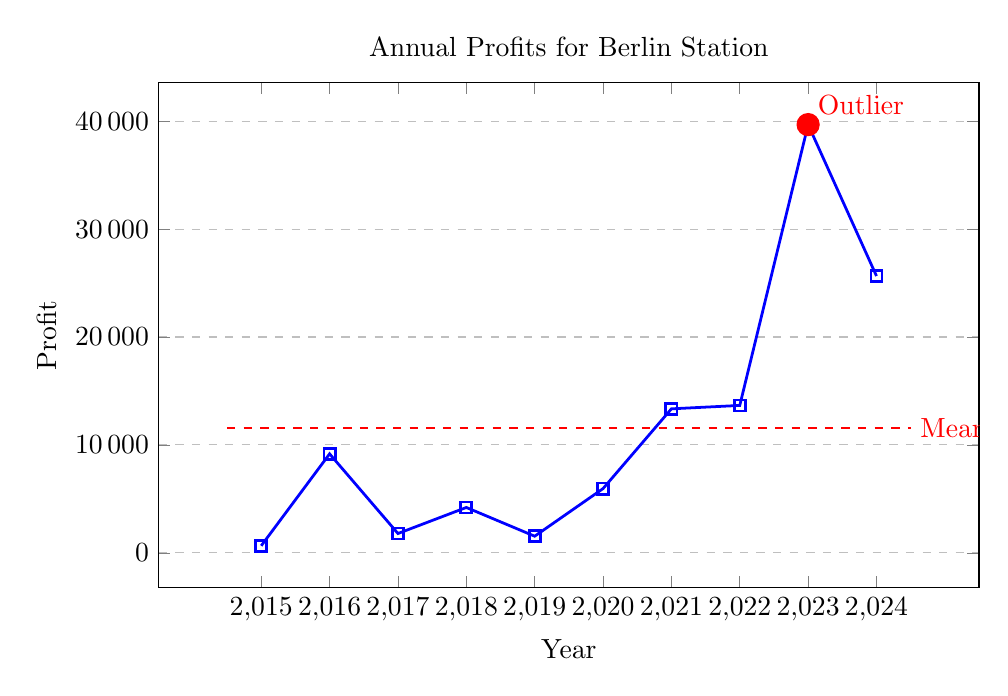
\begin{tikzpicture}
            \begin{axis}[
                title={Annual Profits for Berlin Station},
                xlabel={Year},
                ylabel={Profit},
                xtick={2015,2016,2017,2018,2019,2020,2021,2022,2023,2024},
                scaled y ticks=false,
                y tick label style={/pgf/number format/.cd, fixed, fixed zerofill, precision=0, 1000 sep={\,}},
                ymajorgrids=true,
                grid style=dashed,
                width=12cm,
                height=8cm
            ]

                \addplot[
                    color=blue,
                    mark=square,
                    line width=1pt
                ]
                coordinates {
                    (2015,655.76)
                    (2016,9174.78)
                    (2017,1790.51)
                    (2018,4205.17)
                    (2019,1541.99)
                    (2020,5954.08)
                    (2021,13345.73)
                    (2022,13660.99)
                    (2023,39684.90)
                    (2024,25653.68)
                };

% Add mean line
                \addplot[red,dashed,line width=1pt] coordinates {(2014.5,11566.76) (2024.5,11566.76)};
                \node[red] at (axis cs:2024.5,11566.76) [anchor=west] {Mean};

% Add outlier marker
                \addplot[only marks,mark=*,mark size=4pt,color=red] coordinates {(2023,39684.90)};
                \node[red] at (axis cs:2023,39684.90) [anchor=south west] {Outlier};

            \end{axis}
        \end{tikzpicture}
        \caption{Visualization of Berlin Station Annual Profits with Mean and Outlier Highlighted}
        \label{fig:berlin_profits}
    \end{figure}

    \section{Analysis and Interpretation of Results}
    \subsection{Profitability Patterns and Economic Cycles}
    The mean annual profit of 11,566.76 establishes a baseline performance level against which individual years can be measured. The standard deviation of 12,486.26 indicates moderate volatility, suggesting that while the station experiences fluctuations, its financial performance remains relatively stable over time.

    \subsection{Implications for Infrastructure Investment}
    The profit analysis has direct implications for infrastructure investment decisions. The stability of profits, as indicated by the relationship between mean and median values (11,566.76 vs. 7,564.43), suggests a relatively predictable financial performance that could support long-term investment planning. The slightly higher mean compared to the median indicates a positive skew in the profit distribution, suggesting occasional high-performance periods that pull the average upward.

    \subsection{Statistical Significance and Decision Support}
    The identified outliers and profit extremes provide statistically significant information for decision-making processes. The IQR-based outlier detection method offers a robust approach to identifying exceptional performance periods that warrant further investigation.

    \section{Conclusion}
    The implemented analysis provides a comprehensive statistical overview of railway station profits. The tool allows for interactive exploration of different stations, making it valuable for transportation network managers and analysts.

    Key insights that can be derived from this analysis include:
    \begin{itemize}
        \item Understanding the central tendency and variability of profits
        \item Identifying abnormal profit years that may warrant further investigation
        \item Determining the best and worst performing years
    \end{itemize}

    The broader interpretation of these results within transportation economics and infrastructure management contexts enhances their practical utility, transforming raw statistical outputs into actionable insights for decision-makers. By combining robust statistical methodology with economic interpretation, this analysis provides a solid foundation for data-driven management of railway station networks.


    \appendix
    \section{Code Documentation}
    \subsection{Full Source Code}
    The complete source code for the analysis is available in the project repository. Key components include:
    \begin{itemize}
        \item statistical-analysis.ipynb: Main analysis function
        \item README.md: Usage instructions
        \item Stations\_Data.csv: The dataset used for the analysis
    \end{itemize}

    \section{Data Dictionary}
    \begin{table}[H]
        \centering
        \begin{tabular}{@{}lp{10cm}@{}}
            \toprule
            \textbf{Column} & \textbf{Description} \\
            \midrule
            Station & Name of the railway station \\
            Year & Year of the record \\
            Month & Month of the record \\
            Revenues & Monthly revenue in currency units \\
            Expenses & Monthly expenses in currency units \\
            Profit & Calculated as Revenues - Expenses \\
            \bottomrule
        \end{tabular}
        \caption{Data Dictionary for Stations\_Data.csv}
        \label{tab:data_dictionary}
    \end{table}

    \section{Statistical Formulas}
    \begin{table}[H]
        \centering
        \begin{tabular}{@{}lp{10cm}@{}}
            \toprule
            \textbf{Statistic} & \textbf{Formula} \\
            \midrule
            Mean & $\bar{x} = \frac{1}{n}\sum_{i=1}^{n}x_i$ \\
            Standard Deviation & $\sigma = \sqrt{\frac{1}{n}\sum_{i=1}^{n}(x_i - \bar{x})^2}$ \\
            Median & Middle value of ordered data (50th percentile) \\
            Mode & Most frequently occurring value \\
            Interquartile Range (IQR) & $\text{IQR} = Q_3 - Q_1$ \\
            Outlier Bounds & Lower: $Q_1 - 1.5 \times \text{IQR}$; Upper: $Q_3 + 1.5 \times \text{IQR}$ \\
            \bottomrule
        \end{tabular}
        \caption{Summary of Statistical Formulas Used in Analysis}
        \label{tab:stat_formulas}
    \end{table}

\end{document}